\newcommand{\hex}[1]{\,\texttt{#1}\,}
\newcommand{\temp}{SPLICE\_TEMP }

Before we can discuss operation algorithms correctly, it is useful to first discuss a few features of HBase, and how we make use of them.

In SpliceMachine, we treat HBase rows as sorted Key-Value pairs, which have the following elements:
\begin{enumerate}
\item Row Key $R$, an arbitrary byte array
\item Value Column $V$, an arbitrary byte array
\item Commit Timestamp Column $C$
\item Tombstone Column $T$
\item Anti-Tombstone Column $A$
\end{enumerate}
The commit timestamp, tombstone, and anti-tombstone columns are (for the most part) related to SpliceMachine's transactional implementation--for more information, see our documentation on Transactions. For the purposes of this chapter, we consider only the row key and the value column.

Rows in HBase are sorted in \emph{unsigned lexicographic byte order}. For example, if there are two row keys $R_1 = [0x00 0xEF]$ and $R_2 = [0x00 0xF0]$, then $R_2 > R_1$ because $0xF0 > 0xEF$ when compared in an unsigned manner.

We make extensive use of this sorting property to ensure both correctness and performance. For performance, this sorted-rows feature is used in primary keys and indices to provide sorted table structures, and parallel algorithms which write data into our temporary storage are able to make use of this to provide correctness guarantees.

\section{Encoding Format}
Because we seek to make use of the sortable nature of HBase's row keys, we have to ensure that anything we put in the row key has a lexicographic sort order. More precisely, we must ensure that \emph{any} column which is placed in an HBase column is encoded in such a way as the natural sort order of that data type is the same as its lexicographic sort order. For example, the natural sort order of ${0,3,4,5,6,10,8,7,2}$ is $0,2,3,4,5,6,7,8,10$. We must ensure that it's binary encoded format will retain this sort order under lexicographic ordering.

In point of fact, we have encodings for the following data types which preserve the property that natural sort order is equivalent to lexicographic sort order:

\begin{enumerate}
\item Tinyint
\item Smallint
\item Integer
\item Longint
\item Real
\item Double
\item Float
\item Decimal/Numeric
\item Char
\item Varchar
\end{enumerate}

and throughout this document, we will make use of the notation $enc(t)$ to be the sorted binary encoding for column $t$'s data type.

\subsection{Descending Order Encodings}
Our encoding algorithms will encoding data in ascending order by default. This is acceptable for many situations, but occasionally it is desirable to sort in descending order instead. This, as it turns out, is quite trivial to acheive.

Consider a a byte array containing data in sorted order. We wish to transform that into a byte array representing the reversed order. Thus, we need a transformation $d(x)$ that accepts a byte and generates the reverse of that byte--e.g. $d(x) = x^\wedge{}\hex{0xFF}$.

Therefore, if we take $x^\wedge{}\hex{0xFF}$ for every byte in the ascending order encoding, we will generate the descending-order encoding of the data element.

\section{Packed Encoding}
HBase has a peculiar on-disk storage format that trades inefficiency on disk for efficient random access. In particular, HBase duplicates the row key for every column on the row. For example, if the HBase row has all 4 SpliceMachine columns, then the Row key will be stored 4 times. 

This format is rather inefficient for sequential scanning, however, because it massively increases the amount of data that must be read off disk (particularly for large row keys). To avoid this excessive duplication, SpliceMachine \emph{packs} data into a single column --that is, all data for a single row is stored in a single byte array, using the hex value $\hex{0x00}$ as a field separator.

Because $\hex{0x00}$ is our field separator, its appearance inside any of our encoded fields will mean an incorrect decoding of that row\footnote{which is only a problem if we actually want our rows to decode properly}. Unfortunately, several of our encoding structures have unavoidable occurences of $\hex{0x00}$ within them. This particular situation is a problem for three encodings:

\begin{enumerate}
				\item scalar fields (Tinyint, Smallint, Integer,Longint, Date,Time, and Timestamp)
				\item float fields (Real, Float($p$) where $p\leq23$)
				\item double fields (Double, Float($p$) where $p > 23$)
\end{enumerate}

These fields require special processing in order to properly parse rows. All other data types are guaranteed by encoding to never generate $\hex{0x00}$, and therefore do not require special consideration.

\section{Sparse Versions and Column Indexing}
In our neverending quest to improve I/O efficiency, we wish to avoid recording data repeatedly that does not change. Thus, consider the following

\begin{exmp}[Updating a Row Resulting in data duplication]
				Suppose that Alice inserts row $R = (a,b,c,d)$ into a table and commits. Now suppose Bob wishes to update this row to change the value of $a$ to $z$. In order to properly resolve the row, Bob does the following:

				\begin{enumerate}
								\item Bob reads $R = (a,b,c,d)$ into memory
								\item Bob replaces $a$ with $z$, resulting in $R = (z,b,c,d)$
								\item Bob writes $R$ back.
				\end{enumerate}
				At the end of this operation, SpliceMachine contains two versions of $R$: $(a,b,c,d)$ and $(z,b,c,d)$, which means that $b,c$ and $d$ are all written twice.
\end{exmp}

To avoid this situation, SpliceMachine implements \emph{Sparse Storage}. Instead of each version of a write storing all columns, each version only stores the columns which have \emph{changed} from the previous version. So, considering the same example:

\begin{exmp}[Updating a Row With Sparse Storage]
				Suppose that Alice inserts row $R = (a,b,c,d)$ into a table and commits. Now suppose Bob wishes to update this row to change the value of $a$ to $z$. In order to properly resolve the row, Bob does the following:

				\begin{enumerate}
								\item Bob inserts $R_2 = (z)$
				\end{enumerate}
				At the end of this operation, SpliceMachine contains two versions of $R$: $(a,b,c,d)$ and $(z)$. All data points are only stored a single time.
\end{exmp}

This approach eliminates duplicate data points for rows which have been updated, but at a cost. It is now the responsibility of the reader to ensure that columns are read from the version that they are modified. This is more clearly illustrated by this 

\begin{exmp}[Reading a Sparsely-Stored Row]
				Consider the Row $R$ which has two versions $R_1 = (a,b,c,d)$ and $R_2 = (z)$. Bob wishes to read this row; to do so, he follows this sequence of events:

				\begin{enumerate}
								\item Bob initialized $R_r = (NULL,NULL,NULL,NULL)$
								\item Bob reads $R_2$, since it has the highest timestamp
								\item Bob places $z$ into field 1, giving $R_r = (z,NULL,NULL,NULL)$.
								\item Bob reads $R_1$
								\item Bob places $b,c,d$ into the proper fields, resulting in $R_r=(z,b,c,d)$.
								\item Bob returns $R_r$
				\end{enumerate}
\end{exmp}

This is a fine example in principle, but it leaves out two major issues.

The first issue (which bears on the second issue) is how the reader actually determines which columns are present on each version of a row. To resolve this issue, SpliceMachine prepends a \emph{Column Index}\footnote{In the code it is referred to as a \emph{BitIndex}; this name is a bit confusing, so this document prefers the term Column Index.} to the front of the row's byte array. 

The Column Index determines which columns in the row are present in that particular byte array. The reader then uses this index to properly populate the final row in one pass through each relevant version, stopping when the desired row fields have been completely populated.

Since the Column Index determines which columns are present, the reader can simply skip from $\hex{0x00}$ to $\hex{0x00}$ until the entire row is parsed, or early termination is desired\footnote{E.g. if a predicate fails to match, or if no more columns are desired}. However, if the column to be skipped is a scalar, double, or float type, $\hex{0x00}$ may be contained in the data itself.

To resolve this situation, the Column Index includes information on the data type of the column itself. This information is confined to two bits--whether the column is scalar, float, double, or "other"(e.g. anything else). Thus, the index will also determine whether or not the column requires special logic in parsing.

as of v0.5, the Column Index can come in one of three types: 

\begin{description}
				\item[DenseUncompressed] indices use 1 bit for every column in the row. If that bit is 0, the column is not present. If it is 1, the following 2 bits are the type information
				\item[DenseCompressed] uses Run-length encoding to say, in essence, "the next 4 columns are scalar". It encodes 2 bits for the type, then uses Elias Delta Coding to encode the number of columns which contains that type.
				\item[Sparse] indices use Elias Delta Coding to encode the physical index of the column, then 2 bits additional to store the column type.
\end{description}

Column Indices are typically represented using the notation 

\begin{displaymath}
				C = \{(p(a),t(a)) | \text{a present in the row}\}
\end{displaymath}
where $t(a)$ is the type of column $a$, and $p(a)$ is the column number for $a$(starting from 0).

\subsection{Implicit and Explicit Nulls}
Because the storage is sparse, fields which are not explicitly written are not explicitly stored. This means that, in the case of an update, the value for that column is read from prior versions of the data. 

If the version is the last available version, though, the reader has no choice but to accept any columns which have not been populated as $NULL$ values. This allows an optimization--we have no need to record when a column value is null. Instead, we can ensure that it is considered \emph{absent}, and therefore null, if no version of the row has an explicit value for it.

However, if a user explicitly sets a value to $NULL$, then SpliceMachine \emph{will} explicitly record that column as null. This allows one to set columns to be null which were previously set to a non-null value.

\subsection{Predicate Checking}
Because our data types are encoded using a sortable encoding, it is possible to check some predicates directly against the relevant byte arrays. In particular, ordering predicates (less-than, greater-than, equals, etc.) and null predicates (is null and is-not-null checks) can be converted into direct byte array comparisons. These predicates are significantly less expensive because they do not require decoding.

Additionally, Predicate checking can terminate the row before it has been fully populated. Once a predicate fails to pass, the row can be discarded, even if the row has not been fully decoded. Thus, we can use these byte predicates for added efficiency in our filters.

\section{Table Storage Format}
We have two fundamental types of tables: Sorted, and Unsorted Tables. 

Sorted tables can be either unique or not. Uniquely sorted tables include tables with primary keys, and unique indices. As of v0.5, only non-unique indices are sorted but lack a unique constraint\footnote{An interesting future feature would be an equivalent of a non-unique primary key table.}

\subsection{Uniquely Sorted Tables}
The main advantage of a sorted table is that we can substantially reduce the number of rows that must be checked when performing a qualified scan of the relevant table. Unfortunatly, the main disadvantage of a sorted table is that the distribution of data across a cluster is not required to be uniform, while an unsorted table will.

\begin{exmp}[Sorted Table Row Key Format]
Suppose that table $T$ has columns $(a,b,c,d)$, and has primary keys $(c,a)$. Then the row key is

\begin{align*}
R &= enc(c)\hex{0x00}enc(a)\\
\end{align*}
\end{exmp}

When this is done, we have a table which is sorted according to the sort keys \emph{in ascending order}. Scans which have a predicate on these primary keys can be used to dramatically limit the number of rows which must be processed.

Notice that this structure means that two writes with the same keys would go to the same location in HBase, leading to ambiguous results for that row\footnote{Transactional isolation dictates that these two writes must occur sequentially, otherwise a Write/Write Conflict would be thrown.}. In order to avoid this, SpliceMachine imposes a uniqueness constraint--before a row can be written to a sorted table, SpliceMachine will first check that the row does not already exist, and if it does it will return a Unique Constraint violation.

It is possible to create a unique index which has \emph{descending order}. In order to do this, we simply reverse the bits in the row key.

The data which is actually stored in the value column differs between primary keys and unique indices. Primary keys store the data for all non-primary-key columns, while unique indices will store an encoded version of the row key on the main table.

\subsection{Nonunique Indices}
Non-unique indices function similar to Unique indices, except that they also allow duplicate entries. To allow this, the row key format is slightly different:

\begin{exmp}[Non-unique Indexed Table Format]
Suppose that table $T$ has columns $(a,b,c,d)$ and has an index $I(T)$ on columns $(d,a)$. Then data is stored in $T$ as

\begin{align*}
				R	&=R_{main} \\
V	&= enc(a)\hex{0x00}enc(b)\hex{0x00}enc(c)\hex{0x00}enc(d)
\end{align*}
where $R_{main}$ is the row key in the main table.

The index $I(T)$ is stored as

\begin{align*}
				R &= enc(d) \hex{0x00} enc(a) \hex{0x00} R_{main}\\
\end{align*}
and $V$ is empty
\end{exmp}

\section{Unsorted Tables}
Unsorted tables are the default in SpliceMachine. Whenever there are no primary keys on the table, there is no information which can be placed in the row key (otherwise, the information placed would impose an ordering, and hence result in a primary key). Thus, we use an 8-byte UUID to generate the row key, instead of effective data.
\subsection{Snowflake}
\emph{Snowflake} is the name of the algorithm which generates 8-byte timestamp-based UUIDs\footnote{Credit for the fundamental algorithm goes to Twitter's Open Source project of the same name. We just took the basic algorithm and modified it for our purpose.}

The algorithm is simple: store 64 bits of information using timestamps, counters, and machine ids.

First, we need to enforce uniqueness in time--that is, that the same process cannot generate the same uuid twice in a row. To do that, we use 41 bits of timestamp information--specifically, the lower 41 bits of the 64-bit epoch time(milliseconds since January 1, 1970). This results in $2^{41}$ unique values, or $\approx 69.7$ years worth of unique identifiers, but limits us to only one uuid every millisecond. 

To avoid this annoying rate limit, we add in an 11-bit counter field. This counter takes values between $0$ and $2048$($2^{11}$). If two requests arrive within the same millisecond, then the counter value is incremented to prevent the two requests from overlapping. 

This allows 2048 distinct values to be generated every millisecond by the same process. Once all 2048 possible counters are taken, the process is forced to block requests until the system clock records a new millisecond. 

Finally, we must be unique across multiple machines. Thus, we add a 12-bit \emph{machine id}, which is a preconfigured value between 0 and $2^{12} = 4096$, which uniquely identifies the process which created the UUID generator.

For our purposes, we want unordered UUIDs which are uniformly distributed. Thus, we order our three fields as
\begin{enumerate}
\item 11-bit counter
\item 41-bit timestamp
\item 12-bit machine id
\end{enumerate}

There are three significant restrictions that should be noted.

First, a single Snowflake Generator cannot generate more than 2048 uuids in a single millisecond--once the counter has taken all its available values, the generator must wait for a new timestamp. This means that the maximum throughput for any single Snowflake generator is 122,880,000 UUIDs every second. To get higher throughput than that, multiple Generators must be used, but it's unlikely that most systems will need more than 122 million UUIDs in a single second.

More importantly, the 12-bit machine id means that at more 4096 separate generators can be created in the \emph{entire} SpliceMachine cluster. In practice, this limits the number of RegionServers that an individual SpliceMachine cluster can have to 4096 RegionServers. This is significantly higher than the largest known HBase cluster\footnote{Mobile analytics company Flurry has a cluster with $\approx 1200$ nodes[citation needed], and claim that this is the largest HBase cluster in deployment.}, but it is a limitation all the same.

Most important of all, however, is the timestamp restriction. Because timestamps are an essential part of this algorithm, and we use system clocks to generate timestamps, our generation scheme is highly sensitive to changes in the system clock. If the system clock moves backwards (which can happen unless the system administrator is careful to prevent it), then time is effectively repeated for that process, which will cause duplicate UUIDs to be generated. The Snowflake algorithm will attempt to detect and throw an error when that occurs, but it cannot guarantee to detect changes in all cases. As a result, it is \emph{vitally} important that \emph{all} SpliceMachine clusters be running ntp in a mode that does not move time backwards\footnote{ntpd is one such mode}.

\section{Operation Separation}
Having discussed Table structures, it is now the time to discuss how various operations are actually implemented inside of SpliceMachine. In particular, we would like to know when SpliceMachine executes an operation concurrently, and when it chooses to execute sequentially.

It is usually best to consider a sample query before discussing anything in a more general way. To do so, consider the query 

\begin{lstlisting}[frame=single,captionpos=b,caption=Simple Aggregate Query,language=SQL]
select count(*) from foo
\end{lstlisting}

This query can be visualized as an \emph{execution tree} as in Figure \ref{fig:countTree}.

\begin{figure}
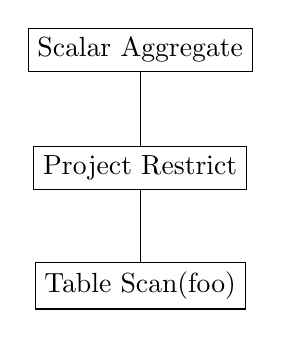
\begin{tikzpicture}[level/.style={sibling distance=60mm/#1}]
\node[rectangle,draw] (z){Scalar Aggregate}
		child { node[rectangle,draw] (b) {Project Restrict}
			child { node[rectangle,draw] (c) {Table Scan(foo)} }
};
\end{tikzpicture}
\caption{Operation Tree for simple count(*) query}
\label{fig:countTree}
\end{figure}

This operation needs to be applied to all regions for the table. It can be performed sequentially--just scan all the rows and count them one by one. Unfortunately, this sequential scanning is very slow for large data sets--we'd like to parallelize it as much as possible.

An alternative is to use a two-stage processing algorithm similar to MapReduce. In this situation, we know that we have multiple independent units of data--specifically, HBase regions. We can compute a separate intermediate count for each region in parallel, and then sum all the intermediate counts sequentially in order to generate our final count.

Now consider a slighty more complex example. Suppose that we are executing the sql
\begin{lstlisting}[frame=single,captionpos=b,caption=Aggregate over join,language=SQL]
select 
	count(*) 
from 
		foo f,
		bar b
where f.foo = b.foo
\end{lstlisting}
This query plan breaks down to the Operation Tree seen in figure \ref{fig:countOverJoinTree}.

\begin{figure}
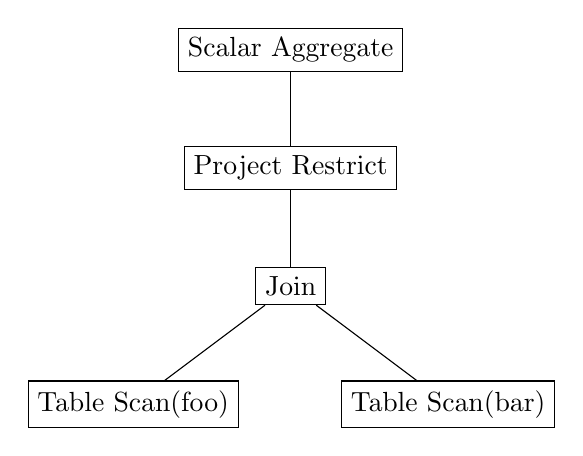
\begin{tikzpicture}[level/.style={sibling distance=120mm/#1}]
\node[rectangle,draw] (z){Scalar Aggregate}
		child { node[rectangle,draw] (b) {Project Restrict}
		child { node[rectangle,draw] (c) {Join}
			child { node[rectangle,draw] (d) {Table Scan(foo)} }
			child { node[rectangle,draw] (e) {Table Scan(bar)} }
	}
};
\end{tikzpicture}
\caption{Operation Tree for Aggregating over a Join}
\label{fig:countOverJoinTree}
\end{figure}

This is harder to imagine an efficient parallelization. Suppose that we could manage to parallelize the join\footnote{Which we can using Merge Sort Join}. In this case it makes more sense to do three stages

\begin{enumerate}
\item Join tables, placing output into intermediate storage
\item generate intermediate counts for joined values
\item merge intermediate counts to generate final results.
\end{enumerate}

This roughly encapsulates the main structure for parallelization in SpliceMachine

\subsection{Splitting Operations}
Given a SQL statement, we always compute an Operation tree that performs our pysical operations, so it's more convenient to discuss operation trees directly than it is to talk about SQL statements themselves.

We define an \emph{operation} as a node within an operation tree. An operation is either \emph{parallel} or \emph{sequential}. A Sequential operation is \emph{not} amenable to parallel execution--it will always be performed sequentially over rows one row at a time.

A Parallel operation, by contrast, is designed to execute in two stages: a \emph{parallel}\footnote{sometimes also referred to as a \emph{sink}} phase, and a \emph{sequential}\footnote{sometimes referred to as a \emph{scan}} phase. 

The parallel phase is strictly confined. During the parallel phase, the operation can take in rows from operations below it, and the output of the operation is written directly to storage\footnote{usually temporary storage, but it's not always required}. 

After all tasks involved in the parallel phase complete, the sequential phase begins (assuming that the operation has a sequential phase).

Thus, we can consider an operation tree as a tree of Sequential and Parallel operations. To correctly execute this tree, we perform a depth-first execution of parallel stages. Each parallel phase encompasses all sequential operations between the parallel operation and the previous parallel operation (or the bottommost operation on the tree). All parallel operations which are lower on the tree \emph{must} complete their parallel phases before the next lowest parallel operation can begin.

So, considering the join example as in Figure \ref{fig:countOverJoinTree}, we see that we have two parallel operations: the Join operation and the Scalar Aggregate. To execute this, we first execute the Join's parallel phase. We thus proceed in a depth-first manner. Since the Join is below the Scalar Aggregate, we execute the Join's parallel operation, writing its intermediate output to a temporary space. This is equivalent to a tree as in Figure \ref{fig:parallelJoinTree}

\begin{figure}
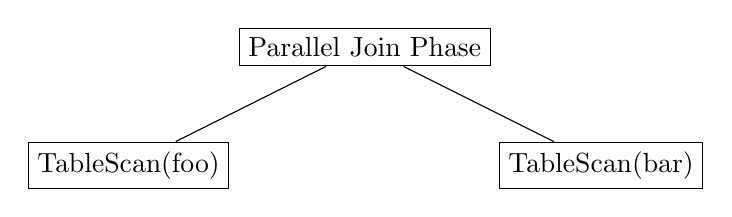
\begin{tikzpicture}[level/.style={sibling distance=60mm/#1}]
\node[rectangle,draw](z){Parallel Join Phase}
	child {node[rectangle,draw](a) {TableScan(foo)}}
	child {node[rectangle,draw](b) {TableScan(bar)}}
;
\end{tikzpicture}
\caption{Operation Tree for a Parallel Join}
\label{fig:parallelJoinTree}
\end{figure}

We execute this tree in parallel, one instance for each Task that we submit. The output of this tree is written into intermediate storage, and then we proceed to the next tree to execute, as in Figure \ref{fig:parallelAggOverJoin}.

\begin{figure}
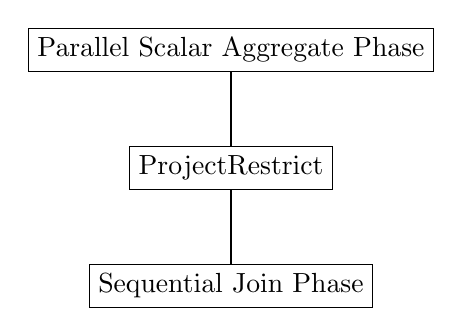
\begin{tikzpicture}[level/.style={sibling distance=60mm/#1}]
\node[rectangle,draw](z){Parallel Scalar Aggregate Phase}
	child {node[rectangle,draw](a) {ProjectRestrict}
	child {node[rectangle,draw](b) {Sequential Join Phase} }
}
;
\end{tikzpicture}
\label{fig:parallelAggOverJoin}
\caption{Operation Tree for Aggregate over Join}
\end{figure}

We can repeat this procedure for arbitrarily complex operation trees (and hence arbitrarily complex SQL statements), and it allows us to execute operations using massive parallelization, while still generating correct sequential results in the end.

\section{TEMP Space}
In order to execute operation trees in the manner we just described, we must have a location where we can store intermediate results. In SpliceMachine\footnote{as ov v0.5. Future versions may eliminate or change this} we use an HBase table called \temp as our intermediate storage.

\temp is an HBase table like any other, which retains data in sorted order, with a few specific modifications.

First, \temp has a different compaction strategy than other tables. Because data is made to exist in \temp for only the length of time taken to perform the next query(or return results to the client), we have no need to compact this data into new files for future IO. As a consequence, when compaction occurs, we only retain store files which contain data for queries which are currently active--all other data is ignored. This leads to hyper-efficient compactions.

Secondly, and far more importantly, \temp is split into $N$ buckets\footnote{The current implementation is to have $N=16$, but future implementations will likely make this more flexible}. These buckets allow some operations to keep data in sorted order without incurring the performance penalty of inserting into a sorted table.

\section{Operation Implementations}
This section describes the various algorithms chosen for the major operations.

\subsection{Parallel Operations over non-scan queries}
All parallel operations require that there be a scan to execute before they can submit tasks (and thus actually be parallel). If the underlying data structure does not have a relevant HBase table (e.g. a values() clause), then the parallel task will become sequential over the in-memory representation.

\subsection{Table Scans}
Table scans are the most fundamental operation in SpliceMachine--nearly all operations require a table scan at one point or another. Its purpose is simple--to scan data in a transactional manner, and to apply any predicates at the lowest possible level.

The basic implementation is sequential: data is scanned in the sort order of the table. As rows are visited, predicates are applied to determine whether or not this row should be included in the output.

For our purposes, a \emph{predicate} is a clause in a query which limits the amount of data which is returned. For example, $a=10$ is a predicate.

When a table is sorted, and a predicate is applied to the sort key \emph{in order}, then the table scan will bound the underlying HBase scan so that fewer rows will be visited. 

\begin{exmp}[Bounding a TableScan with a sort predicate]
Suppose $T$ is a table with columns $(a,b,c,d)$, and primary key $(b,a)$. Then, consider the SQL

\begin{lstlisting}[frame=single,captionpos=b,caption=SQL for bounded scan,language=SQL]
	select * from T where b = 10 
\end{lstlisting}

				This SQL will construct a table scan which is bounded so that only rows which have keys in the range $[10,11)$ are considered.

				By contrast, the sql

\begin{lstlisting}[frame=single,captionpos=b,caption=SQL for unbounded scan,language=SQL]
	select * from T where a = 10 
\end{lstlisting}
				will not be able to bound the rows--it must interact with every row in $T$ to determine the correct result
\end{exmp}

Predicates are applied at the byte level--data is \emph{not} decoded in order to check predicates. Instead, values are encoded into byte arrays, and the comparison is performed using lexicographic sort order\footnote{This is the primary reason why data is encoded in sorted order}.

It is important to note that (as of v0.5) Table scans are \emph{not} parallel operations. While the application of predicates \emph{could} be parallelized, Table scans are assumed to be short(in which case it is more efficient to perform a sequential scan), bounded by a sort order(either a primary key or an index), or underneath a parallel operation. In any of these three cases, a parallel Table scan operation would pose a performance penalty. However, this does mean that full table scans which are not under another parallel operation will take time linear in the number of rows. 

\subsubsection{Multi-probe scans}
When a table is sorted via a primary key or index, and the keyed columns are used in a SQL \emph{in} clause (where a key is allowed to match one of several values), then the table scan may produce a \emph{Multi-probe Scan}.

A Multi-probe scan is a table scan which has multiple separate bounding scans. Thus, it is possible to create multiple scans, each only responsible for scanning data which matches one entry in the clause.

\begin{exmp}[Multiple Bounds on a table scan]
Suppose $T$ is a table with columns $(a,b,c,d)$, and a primary key $(b,a)$. Then, consider the SQL

\begin{lstlisting}[frame=single,captionpos=b,caption=SQL for multiple bounds,language=SQL]
	select * from T where b in (10,15) and a = 5
\end{lstlisting}
Then the table scan is a multi-probe scan with two scans: $[10,11)$ and $[15,16)$, each of which will apply the $a=5$ predicate.
\end{exmp}

This technique can be used with an arbitrarily large number of entries in the \emph{in} clause. Be aware, however, that this may result in a massive increase in the number of tasks that need to be executed for parallel scans, which may incur a performance penalty.

\subsection{Index lookups}
Indices typically do not contain all the columns in a table\footnote{When they do, they are referred to as \emph{covering indices}}, so in order to fill some queries, an index lookup must be performed.

Index lookups in SpliceMachine are exceptionally expensive, because each request must go across the network to another table (potentially another server).

To avoid the network cost for every row, SpliceMachine batches up index lookups, and performs an HBase \emph{multi-get} to fetch multiple rows in bulk. To further reduce latency, SpliceMachine also performs \emph{forward fetches}--it uses a background thread to fetch the next batch of rows before it is requested.

Index lookup operations are usually referred to by their Derby reference, as \emph{IndexRowToBaseRow} or just \emph{IndexRow} operations; they are all sequential operations, designed to fit within a larger operation tree.

\subsection{ProjectRestrict}
There are two forms of operations which are done to transform and limit data in ways which are not amenable to raw table scans.

One operation is referred to as a \emph{projection}. Projections are transformations of the data, such as dividing two numbers, or computing substrings, etc. 

Another operation is referred to as a \emph{restriction}. Restrictions are mechanisms for filtering out rows which do not match predicate, but whose predicate is too complex to be converted into a scan qualifier.

In SpliceMachine, These two tasks are constructed in a single \emph{ProjectRestrict} operation. ProjectRestrict operations are sequential, and operate against a single row at a time.

\subsection{Aggregation}
Aggregation is a central theme of many SQL queries. In SpliceMachine, aggregation comes in four major forms:

\begin{description}
				\item[Scalar Aggregates] take in many rows, and output exactly one result.
				\item[Grouped Aggregates] emit one row per \emph{grouping key}
				\item[Distinct Scalar Aggregates] remove duplicate rows, then perform a scalar aggregate.
				\item[Distinct Grouped Aggregates] remove duplicate entries, then perform a grouped aggregate.
\end{description}
\subsubsection{Scalar Aggregates}
Scalar aggregation is a parallel operation, which aggregates \emph{all} matching rows into a \emph{single} row value. 

The parallel phase of a scalar aggregation consists of reading all data from its subtree, and aggregating the result. When its subtree runs out of rows, the aggregated value is finalized and written into \temp. Then the sequential phase of the operation reads the intermediate counts out and merges them together to form a final result.

\subsubsection{Grouped}
Grouped Aggregation is a parallel operation, which aggregates rows around a set of \emph{grouping keys}. 

The parallel phase of the grouped aggregation consists of reading data from its subtree, and placing each row into a hashtable. If the grouping keys already exist in the hashtable, then the row will be merged together to form an aggregated count; if they are not, then the row is added. To avoid overusing memory, this hashtable is bounded; when the number of rows in the hashtable exceeds a threshold, then a row is evicted and written to \temp. The sequential phase will then read each row that is stored in \temp and merge together matching entries.

When the grouped aggregate is underneath another parallel operation, the sequential phase will occur in parallel; in these cases, we'll need to ensure that a single task will need to read all data for a specific key. To perform this, we use a \emph{Region-aware Scanner}. This scanner will read rows off of other regions as necessary to ensure that grouping keys will be treated by one and only one region.

\subsubsection{Distinct Grouped}
Distinct Grouped Aggregates are special cases of Grouped Aggregation, except that duplicate entries are discarded during the parallel phase, rather than aggregated.

Additionally, distinct grouped aggregates will overwrite rows in \temp, which avoid duplication across multiple regions.

\subsubsection{Distinct Scalar}
Distinct Scalar operations is a 2-phase parallel operation. The first phase is identical to a distinct grouped aggregate, while the second phase is equivalent to a scalar aggregation.

\subsection{Sorting}
Sorting is a very simple parallel operation, which writes data into \temp, using the sort keys as row keys, then reading data out of \temp.

Distinct sorting is a sort model that is similar to Distinct Grouped aggregation, but without the final merge step. In effect, it throws away duplicate entries, then scans the non-duplicated entries out of \temp.

\subsection{Distinct Scan}
Distinct scanning in SpliceMachine is functionally equivalent to Distinct sorting in SpliceMachine. The only reason it exists is that distinct scan does not \emph{require} sorting (although the implementation will sort in effect).

\subsection{Joins}
Joins come in several varieties, and are useful in different contexts.
\subsubsection{MergeSortJoin}
a MergeSort join is a parallel operation which is useful for performing joins against two large tables which are not sorted according to the join key.

The MergeSort Join algorithm is simple. In the parallel phase, the left and right sides of the table are scanned in parallel, and written to \temp. The row key in \temp are the join keys, plus a \emph{join ordinal}, which is a 1-byte entry determining which side of the join the row came from. This ordinal is such that right-side rows are sorted before left-side rows. Then, during the sequential phase, all right-side entries \emph{for a single join key} are read into memory. After this occurs, all left-side rows which match taht join key are read.

MergeSortJoin requires that only the right side rows \emph{for a given key} fit within memory\footnote{This does not mean that the right hand side must fit completely within memory, only that the rows needed to join to a single left-hand-side row do.}. This makes it effective when both tables to be joined are very large and are not sorted according to the join keys. If the right-hand-side is very small, then Broadcast joins are more effective; if the two tables are both sorted according to the join keys, then MergeJoin is more appropriate\footnote{In most cases. MergeJoin is not parallel, however, so some queries will not perform well when using straight MergeJoins}.

\subsubsection{MergeJoin}
MergeJoin is a sequential equivalent of MergeSortJoin, in that it reads data from two sorted locations; it is different in that it assumes that both the left and right side of the join are sorted in the same ordering. When this is satisfied, MergeJoin will open only two scans--one for the right side, and one for the left. It will then merge data together in sequence, just as in the classic MergeSort algorithm.

MergeJoin requires that both tables to be joined are sorted according to the join keys for the query, or else it cannot be used. Within this constraint, however, there is no limitation on the resources available to perform a MergeJoin.

As MergeJoin is \emph{not} a parallel operation, it may be desirable to prefer MergeSortJoin whenever there is high selectivity in the join (that is, that many rows will not match the given join criteria, so the output of the join is very small) and when there are no parallel operations on top of the MergeJoin itself. Otherwise, it is almost always preferable to use MergeJoins whenever possible, as it will avoid the extra cost of sinking data into \temp.

\subsubsection{Broadcast}
When the right side of a join is extremely small, it is cheaper to pay the penalty to just scan the entire table and then perform the join in memory--these situations form the basis of the Broadcast Join.

Broadcast Joins operate sequentially by first reading the \emph{entire} right-side into the left side's memory space. Then, for each row on the left side, it refers to its memory space for the proper right-side rows.

Broadcast Joins require that the entire right hand side be able to fit within the memory space of the left-hand-side's operating capacity. As there is an initial latency due to reading the right hand side, Broadcasts may perform more poorly than MergeJoins when the right side is large (even if the right side can fit within memory).

Broadcast Joins are \emph{not} parallel operations, so a broadcast join operation will not execute in parallel unless a parallel operation is above it.

\subsubsection{NestedLoopJoin}
NestedLoopJoins are the simplest form of join. It is a sequential operation that executes a join using a "nested loop"; for each left row that is scanned in, a new scan is created for the right side, with the matching qualifiers. A joined row is then created for each row emitted from the right-side scan. When that scan is exhausted, the left side is allowed to proceed to the next row and repeat.

NestedLoopJoins displays very poor performance in most cases, and should be avoided as much as possible. The only situation in which a NestedLoopJoin must be used is for non-equi-joins\footnote{As of v0.5. Future versions may modify Merge and MergeSort joins to perform non-equi-joins} in which the right hand side is considered too large to use a Broadcast join with.


\subsection{Unions}
Unions come in two forms: \emph{Union All} and \emph{Union}. A UnionAll operation will return \emph{all} the rows from the left side with \emph{all} the rows from the right side, while a Union operation will return only the distinct elements which are contained in either the left or the right side.

The query optimizer will rewrite a Union operation as a Distinct Sort over a UnionAll operation, so the only true implementation of Union is the UnionAll.

When a UnionAll is over a table scan, then it will emit all the left rows, then a separate region will emit all the right rows. When both left and right are wholly in memory (i.e. over a values clause), then UnionAll will emit all left then all right within the same java heap.

Since UnionAll is effectively two table scans in sequence, it is implemented as a sequential operation. As Union is effectively a distinct sort, Unions are parallel.

\subsection{DML Write operations}
DML write operations come in three flavors(Inserts, Updates, and Deletes), all of which follow the same basic pattern. Firstly, all DML write operations are parallel--when executed over a scan, they will perform that scan in parallel. However, when the underlying structure does not correspond to a scan (i.e. a values() clause), then the operation is performed sequentially over the in-memory representation.

Secondly, DML write operations do not write to \temp, instead they write to the destination table directly, and those writes are goverened by Snapshot Isolation. Thus, DML write operations may throw a Write/Write Conflict during concurrent access. 

\subsection{Insert}
Inserts are a very straightforward implementation, taking rows from the operation subtree and writing them to the destination table in bulk. If the destination table has a primary key, then Inserts will construct those. Similarly, if there is a sequential field, Inserts will generate the next sequential id for insertion.

\subsubsection{Sequential Column}
SpliceMachine supports (as of v0.5) a limited form of a sequential identifier. However, there are some notable differences between a SpliceMachine sequence and a more traditional sequence.

In a traditional (single-node) database, sequences are fairly trivial to implement-- a durable atomic counter is all that is necessary. However, creating a durable atomic counter which can be accessed by many nodes is a significant challenge, and often imposes a high degree of latency.

To avoid the increased latency\footnote{as of v0.5}, SpliceMachine uses a \emph{partially-ordered} implementation. In this implementation, there is a column on the HBase table $SPLICE\_SEQUENCES$ which is unique for each sequential column in the system. This column stores a long which contains the last \emph{reserved} sequence id.

When a node wishes to use the sequence, it will attempt to \emph{reserve} a block of sequence ids (by default, 1000). This requires a network call to update the column in $SPLICE\_SEQUENCES$. After this call, sequence ids are issued in order until the block is exhausted. When that occurs, the node will attempt to reserve another block, and so on.

Because multiple servers may be executing in parallel, this algorithm means that some rows may appear out of order, and not all sequence ids are guaranteed to occur. However, each sequence id \emph{is} unique, and thus may be used as a primary key (if needed). Note however that using a sequential field as a primary key will result in uneven write performance, as only a few regions at a time will accept writes.

\subsection{Updates}

Updates are a parallel operation which attempts to modify data in place. Under Snapshot Isolation, an Update is actually an insert with a new timestamp, so the functional structures are similar.

As of v0.5, Updates cannot be performed over a parallel suboperation, because the location of the row to be updated is lost during the suboperation's parallel execution phase.

\subsubsection{Updating Primary Keys}
When a primary key needs to be updated, its HBase row key must be changed. However, HBase does not allow the mutation of a row key directly. Instead, the Update operation must delete the old row and then insert the new one. In order to do this, Updates must be sure to acquire all relevant information with which to move the row; this may require a remote hbase GET operation to be performed.

When primary keys are not modified (or there are no primary keys on the table), then an update will behave exactly as if it were an insert.

\subsection{Deletes}
Deletes in SpliceMachines are specialized insertions--an empty byte array is written to the row location, and Snapshot Isolation appends a \emph{tombstone} value to the location, indicating that the row should be considered deleted.

As of v0.5, Deletes cannot be performed over a parallel suboperation, because the location of the row to be deleted is lost during the suboperation's parallel execution phase.

\subsection{Import}
Imports are a specialized procedure in SpliceMachine to efficiently load a large volume of data into the system relatively quickly. They are parallel \emph{in the number of files}--that is, each file to be imported will be granted its own task. 

Files must be stored in HDFS before they may be imported. This is because there is no way of knowing a priori which node will actually perform the import processing (tasks are assigned at random), and because if a task fails, it may be necessary to retry that task on a different node; therefore, the data file \emph{must} be equally accessible to all nodes in the same way, which requires HDFS\footnote{There is often some confusion here, so it is important to emphasize. There is \emph{absolutely no} way that a file stored on local storage of a single machine could be successfully imported except by that machine. If that machine fails, then the import must fail. SpliceMachine has opted for the design of fault tolerance in this case, which means allowing multiple machines access. HDFS is a non-negotiable part of this design. }.

Within a task, there is a single thread which reads data off of HDFS, and then multiple \emph{processor} threads, which take data from the reader thread, parse it into the proper binary representation, and attempt to write that representation to the destination table. In this way, an import is much like an Insert, but where an insert operation requires the underlying operation to be a table scan (and hence already in the proper storage format), Imports require data to be in a user-specified format.

\subsection{Subqueries}
Subqueries are typically implemented as a ProjectRestrict operation, where the ProjectionOperation is the execution of the subquery. This means that, while the subquery \emph{itself} may be a parallel operation, the \emph{full} query may not be.

\section{Appendix: List of Operations}
This appendix is a short list of operations, as well as some brief information about them (whether the operation is parallel or sequential, and what the row key is for \temp if the operation is parallel).

To make this table more concise, we introduce the variables described in Table \ref{tab:op-legend}.

\clearpage
\begin{table}
\begin{tabular}{|l|l|}
				\hline
				\bf{Variable}	&	\bf{Description}								\\	\hline
				$t$			&	Unique Task ID												\\	\hline
				$f$			&	Fixed bucket id												\\	\hline
				$o$			&	Unique Operation ID										\\	\hline
				$uuid$	&	Unique Row ID													\\	\hline
				$g$			& Grouped/Sorting columns								\\	\hline
				$j$			&	Join Ordinal(either left or right)		\\	\hline
				$b(g)$	& Unique bucket for the grouped columns	\\	\hline
\end{tabular}
\\
\caption{Variable definitions for Operation List}
\label{tab:op-legend}
\end{table}

\begin{table}
				\begin{tabular}{|l|c|p{6cm}|}
								\hline
								\bf{Operation}	&	\bf{Is Parallel?}	&	\bf{Output Row Key} \\ \hline

								TableScan													&	No	&	\\	\hline
								Index Lookup											&	No	&	\\	\hline
								ProjectRestrict										&	No	&	\\	\hline
								Union All													&	No	&	\\	\hline
								ScalarAggregate										&	Yes	&	$f|o|uuid|t$				\\	\hline
								GroupedAggregate									&	Yes	&	$b(g)|o|g|uuid|t$		\\	\hline
								DistinctGroupedAggregate					&	Yes	&	$b(g)|o|g$					\\	\hline
								Sort															&	Yes	&	$f|o|g|uuid|t$			\\	\hline
								Distinct Sort											&	Yes	&	$f|o|g$							\\	\hline
								MergeSortJoin											&	Yes	&	$b(g)|o|g|j|uuid|t$	\\	\hline
								DistinctScalarAggregate(Phase 1)	&	Yes	&	$b(g)|o|g$					\\	\hline
								DistinctScalarAggregate(Phase 2)	&	Yes	&	$f|o|uuid|t$				\\	\hline
								Union\tablefootnote{Unions are equivalent to Sort over a Union All}	&	Yes	&	$f|o|g|uuid|t$			\\	\hline
								MergeJoin													&	No	&	\\	\hline
								BroadcastJoin											&	No	&	\\	\hline
								Insert														&	Yes	&	table dependent \\ \hline
								Update														&	Yes	&	table dependent	\\	\hline
								Delete														&	Yes	&	table dependent	\\	\hline
								Import														&	Yes	&	table dependent \\ \hline
				\end{tabular}
				\caption{List Of Operations}
				\label{table:op-list}
\end{table}

%End Operation Execution Chapter
